\documentclass[runningheads]{llncs}
%
\usepackage{graphicx}
\usepackage{xtab}
\usepackage{stmaryrd}
\usepackage{amsmath, amssymb}
\usepackage{listings}
% If you use the hyperref package, please uncomment the following line
% to display URLs in blue roman font according to Springer's eBook style:
% \renewcommand\UrlFont{\color{blue}\rmfamily}

% OUR MACROS
%%%%%%%%%%%%%%%%%%%%%%%%%%%%%%%%%%%%%%%%%%%%%%
%							References
%%%%%%%%%%%%%%%%%%%%%%%%%%%%%%%%%%%%%%%%%%%%%%

\newcommand{\chapref}[1]{Chapter~\ref{#1}}
\newcommand{\appref}[1]{Appendix~\ref{#1}}
\newcommand{\sectref}[1]{Section~\ref{#1}}
\newcommand{\subsectref}[1]{Subsection~\ref{#1}}
\newcommand{\figref}[1]{Figure~\ref{#1}}
\newcommand{\tabref}[1]{Table~\ref{#1}}
\newcommand{\egref}[1]{Example~\ref{#1}}
\newcommand{\eqnref}[1]{(\ref{#1})}
\newcommand{\thmref}[1]{Theorem~\ref{#1}}
\newcommand{\propref}[1]{Proposition~\ref{#1}}
\newcommand{\lemref}[1]{Lemma~\ref{#1}}
\newcommand{\defref}[1]{Definition~\ref{#1}}

\newcommand{\chapchapref}[2]{Chapters~\ref{#1} and \ref{#2}}
\newcommand{\sectsectref}[2]{Sections~\ref{#1} and \ref{#2}}
\newcommand{\figfigref}[2]{Figures~\ref{#1} and \ref{#2}}
\newcommand{\tabtabref}[2]{Tables~\ref{#1} and \ref{#2}}

\newcommand{\sectsectsectref}[3]{Sections~\ref{#1}, \ref{#2} and \ref{#3}}
\newcommand{\figfigfigref}[3]{Figures~\ref{#1}, \ref{#2} and \ref{#3}}

%%%%%%%%%%%%%%%%%%%%%%%%%%%%%%%%%%%%%%%%%%%%%%
%							Code Listings
%%%%%%%%%%%%%%%%%%%%%%%%%%%%%%%%%%%%%%%%%%%%%%

%% Core language
%\lstdefinelanguage{SaltyLang}{
% keywords=[1]{all, any, mutex}
% keywordstyle[1]=\color{Cyan},
% keywords=[2]{controller, where, input, output, enum, env_init, env_trans, env_liveness, sys_init, sys_trans, sys_liveness, def},
% keywordstyle=[2]\color{blue!90!black},%\bfseries,
% keywords=[3]{False, True},
% keywordstyle=[3]\color{ForestGreen},%\bfseries,
% keywords=[4]{all, any, mutex, leads_to, Bool, if, then, else},
% keywordstyle=[4]\color{Cyan},
% otherkeywords={', !, <, ->, <->, \, /, /\\, \\/},
% keywordstyle=\color{Cyan},
% identifierstyle=\color{black},
% sensitive=true,
% comment=[l]{--},
% commentstyle=\color{Magenta}
%}
%
%% Additional options
%\lstset{
% language=SaltyLang,
% basicstyle=\small\ttfamily,
% tabsize = 2,
% numbers=none,
% mathescape=false,
% showstringspaces=false
%}

%%%%%%%%%%%%%%%%%%%%%%%%%%%%%%%%%%%%%%%%%%%%%%
%							Theorem Environments
%%%%%%%%%%%%%%%%%%%%%%%%%%%%%%%%%%%%%%%%%%%%%%

%\newtheorem{lemma}{Lemma}
%\theoremstyle{definition} % turn off pesky italics
%\newtheorem{definition}{Definition}
%\newtheorem{example}{Example}
%\newtheorem{theorem}{Theorem}
%\newtheorem{proposition}{Proposition}
%\newtheorem{proof}{Proof}


%%%%%%%%%%%%%%%%%%%%%%%%%%%%%%%%%%%%%%%%%%%%%%
%							Definitions
%%%%%%%%%%%%%%%%%%%%%%%%%%%%%%%%%%%%%%%%%%%%%%

% Standard sets of numbers
\def\Nset{\mathbb{N}}
\def\Rset{\mathbb{R}}
\def\Zset{\mathbb{Z}}

% Reactive synthesis sets
\def\inputs{\mathcal{I}}
\def\outputs{\mathcal{O}}


% abbreviations
%\def\act{{Act}}
%\def\sinit{{\overline{s}}}

% logical operators
\def\limplies{\rightarrow}
\newcommand{\lequiv}{\leftrightarrow}
\newcommand{\ltrue}{\textrm{true}}
\newcommand{\lfalse}{\textrm{false}}
\newcommand{\lxor}{\oplus}

% temporal operators
\def\always{\square}
\def\until{\mathbin{\mathsf{U}}}
\def\wuntil{\mathbin{\mathsf{W}}}
\def\release{\mathbin{\mathsf{R}}}
\def\eventually{\lozenge}
\def\always{\square}
\def\lnext{\varbigcirc}

\def\palways{\square^{-1}}
\def\peventually{\lozenge^{-1}}
\def\past{\varbigcirc^{-1}}

\newcommand{\talways}[2]{\square^{#1..#2}}
\newcommand{\teventually}[2]{\lozenge^{#1..#2}}
\newcommand{\tuntil}[2]{\mathbin{\mathsf{U}}^{#1..#2}}
\newcommand{\trelease}[2]{\mathbin{\mathsf{R}}^{#1..#2}}


% model checking

%\def\true{{\mathit{true}}}
%\def\false{{\mathit{false}}}
%\def\AP{{\mathit{AP}}}
%\def\Dist{{\mathit{Dist}}}
%\def\Sat{{\mathit{Sat}}}
%\def\Steps{{\mathit{Steps}}}
%\def\sinit{{s_\mathit{init}}}
%\def\Prob{{\mathit{Prob}}}
%\def\Pr{{\mathit{Pr}}}
%\def\Path{{\mathit{Path}}}
%\def\Pathfin{{\mathit{FPath}}}
%\def\Pathful{{\mathit{Path}_\mathit{ful}}}
%\def\Adv{{\mathit{Adv}}}
%\def\calAfair{{{\cal A}_\mathit{fair}}}
%\def\sat{{\,\models\,}}
%\def\notsat{{\,\not\models\,}}
%\def\satAdv{{\,\models_\mathit{Adv}\,}}
%\def\notsatAdv{{\,\not\models_\mathit{Adv}\,}}
%\def\satfair{{\,\models_\mathit{fair}\,}}
%\def\next{{X\,}}
%\def\until{{\ {\cal U}\ }}
%\def\buntil{{\ {\cal U}^{\leq k}\ }}
%\def\tuntil{{\ {\cal U}^{\leq t}\ }}
%\def\sqlt{{\sqsubset}}
%\def\sqleq{{\sqsubseteq}}
%\def\sqgt{{\sqsupset}}
%\def\sqgeq{{\sqsupseteq}}
%\def\psmin{{p_s^\mathit{min}}}
%\def\psmax{{p_s^\mathit{max}}}
%\def\ptmin{{p_t^\mathit{min}}}
%\def\ptmax{{p_t^\mathit{max}}}
%\def\pspmin{{p_{s'}^\mathit{min}}}
%\def\pspmax{{p_{s'}^\mathit{max}}}
%\def\Syes{{S^{\mathit{yes}}}}
%\def\Sno{{S^{\mathit{no}}}}
%\def\Sqm{{S^?}}
%\def\done{{\mathit{done}}}
%\def\calPbp{{\cal P}_{\bowtie p}}
%\def\calSbp{{\cal S}_{\bowtie p}}
%\def\Var{{\mathit{Var}}}
%\def\Act{{\mathit{Act}}}
%\def\glob{{\mathit{glob}}}
%\def\ind{{\mathit{ind}}}
%\def\enc{{\mathit{enc}}}
%\def\etmcc{{ $\mathsf{E} {\;} \rotatebox{90}{$\mathsf{T}$} {\;} \mathsf{MC}^\mathsf{2}$ }}
%\def\implies{{\rightarrow}}

%%%%%%%%%%%%%%%%%%%%%%%%%%%%%%%%%%%%%%%%%%%%%%
%							Commands
%%%%%%%%%%%%%%%%%%%%%%%%%%%%%%%%%%%%%%%%%%%%%%


\newcommand{\pdist}[1]{\mathcal{D}({#1})}
\newcommand{\tfunction}{\longrightarrow}
\newcommand{\trans}[3]{#1 \overset{#2}{\longrightarrow} #3}
\newcommand{\allstates}{\overline{S}}

\newcommand{\allstratstwo}{\Sigma}
\newcommand{\strattwo}{\sigma}
\newcommand{\Rsetinf}{\Rset_{\pm\infty}}
\def\Rset{\mathbb{R}}
\def\Qset{\mathbb{Q}}
\newcommand{\dwc}{\textsf{dwc}}
\newcommand{\mydef}{\stackrel{\mbox{\rm {\tiny def}}}{=}}
\newcommand{\PONE}[1]{\textsf{Player~1}}
\newcommand{\PTWO}[1]{\textsf{Player~2}}
\newcommand{\PLAYER}[1]{\textsf{Player}~${#1}$}
\newcommand{\Exp}{\mathbb{E}}
%\renewcommand{\Pr}{\mathrm{Pr}}
\newcommand{\rew}{\mathsf{rew}}


\def\calPle{{\cal P}_{\le \lambda}}
\def\Pr{{\mathit{Pr}}}
\def\Prps{{\mathit{Pr}_{M^c}^{\sinit}}}


\newcommand{\salty}{Salty\xspace}
\newcommand{\enum}{{\texttt{enum}}\xspace}
\newcommand{\true}{{\texttt{True}}\xspace}
\newcommand{\false}{{\texttt{False}}\xspace}
\newcommand*\necessary{\mathord{\Box}}
\newcommand*\possible{\mathord{\Diamond}}
\newcommand{\sysinit}{\lstinline{sys_init}\xspace}%{{\texttt{sys\_init}}\xspace}
\newcommand{\envinit}{\lstinline{env_init}\xspace}%{{\texttt{env\_init}}\xspace}
\newcommand{\systrans}{\lstinline{sys_trans}\xspace}%{{\texttt{sys\_trans}}\xspace}
\newcommand{\envtrans}{\lstinline{env_trans}\xspace}%{{\texttt{env\_trans}}\xspace}
\newcommand{\sysliveness}{\lstinline{sys_liveness}\xspace}%{{\texttt{sys\_liveness}}\xspace}
\newcommand{\envliveness}{\lstinline{env_liveness}\xspace}%{{\texttt{env\_liveness}}\xspace}


\begin{document}
\lstset{language=Ada}
\lstset{basicstyle=\ttfamily}
%%%%%%%%%%%%%%%%%%%%%%%%%%%%%%%%%%%%%%%%%%%%%%%%%%%%%%%%%%%%%%%%%%%%%%%%%%%%%%%%
% TITLE
%%%%%%%%%%%%%%%%%%%%%%%%%%%%%%%%%%%%%%%%%%%%%%%%%%%%%%%%%%%%%%%%%%%%%%%%%%%%%%%%
%
\title{End-to-End Verification of Initial and Transition Properties of GR(1) Designs in SPARK\thanks{Supported by AFRL contract FA8650-16-C-2642 and AFOSR grant RQCOR20-35.}}
%
\titlerunning{End-to-End Verification of GR(1) Designs in SPARK}
% If the paper title is too long for the running head, you can set
% an abbreviated paper title here
%
%\author{Laura Humphrey\inst{1}\orcidID{0000-1111-2222-3333} \and
%James Hamil\inst{2}\orcidID{1111-2222-3333-4444} \and
%Joffrey Huguet\inst{3}\orcidID{2222--3333-4444-5555}}
\author{Laura Humphrey\inst{1} \and
James Hamil\inst{2} \and
Joffrey Huguet\inst{3}}
%
\authorrunning{L. Humphrey et al.}
% First names are abbreviated in the running head.
% If there are more than two authors, 'et al.' is used.
%
\institute{Air Force Research Laboratory, WPAFB, OH 45433, USA \\
\email{laura.humphrey@us.af.mil} \and
LinQuest Corp., Beavercreek, OH 45431, USA \\
\email{james.hamil.ctr@us.af.mil}  \and
AdaCore, F-75009 Paris, France \\
 \email{huguet@adacore.com}}
%
\maketitle              % typeset the header of the contribution
%
%%%%%%%%%%%%%%%%%%%%%%%%%%%%%%%%%%%%%%%%%%%%%%%%%%%%%%%%%%%%%%%%%%%%%%%%%%%%%%%%
% ABSTRACT
%%%%%%%%%%%%%%%%%%%%%%%%%%%%%%%%%%%%%%%%%%%%%%%%%%%%%%%%%%%%%%%%%%%%%%%%%%%%%%%%
\begin{abstract}
%The abstract should briefly summarize the contents of the paper in 150--250 words.
Manually designing control logic for reactive systems is time-consuming and error-prone. 
An alternative is to automatically generate controllers using ``correct-by-construction'' synthesis approaches. 
Recently, there has been interest in synthesis from Generalized Reactivity(1) or GR(1) specifications, 
since the required computational complexity is relatively low, and several tools now exist for GR(1) synthesis.
However, while these tools implement synthesis approaches that are theoretically ``correct-by-construction,'' 
errors in tool implementation can still lead to errors in synthesized controllers. 
We are therefore interested in ``end-to-end'' verification of synthesized controllers with respect to their original GR(1) specifications.
Toward this end we have modified Salty -- a tool that produces executable software implementations of controllers 
from GR(1) specifications in a variety of programming languages -- to produce implementations in SPARK.
SPARK is both a programming language and associated set of verification tools, so it has the potential to enable the ``end-to-end'' verification we desire.
In this paper, we discuss our experience to date using SPARK to implement controllers and verify them against 
a subset of properties comprising GR(1) specifications, namely system initial and transition properties. 
We also discuss lessons learned about how to best encode controllers in SPARK for verification, 
examples in which verification found unexpected controller behaviors, and 
caveats related to the interpretation of GR(1) specifications.

%In this paper, we discuss our experience to date using SPARK to implement controllers and to verify them against 
%a subset of properties comprising their original GR(1) specifications, in this case system initial and transition properties. 
%There are many ways to encode synthesized controllers in SPARK, so we describe the encoding that we found to be most efficient for verification. 
%We also describe the contracts and assertions that we needed to generate within the controller implementation so that 
%SPARK could verify the aforementioned properties automatically, i.e. without requiring additional annotations from the user.
%We give some preliminary results on the approximate size of controllers that can be verified and the amount of time needed for verification, 
%using a database of GR(1) specification examples pulled from a variety of sources. 
%Finally, we close with a discussion of certain implementation choices that arise due to environment assumptions encoded in GR(1) specifications, 
%some of which we have handled and some of which we have currently deferred. 
%We also discuss possible approaches for verifying the full set of GR(1) properties, i.e. including liveness.

\keywords{Reactive synthesis \and end-to-end verification \and functional verification.}
\end{abstract}

%%%%%%%%%%%%%%%%%%%%%%%%%%%%%%%%%%%%%%%%%%%%%%%%%%%%%%%%%%%%%%%%%%%%%%%%%%%%%%%%
% INTRODUCTION
%%%%%%%%%%%%%%%%%%%%%%%%%%%%%%%%%%%%%%%%%%%%%%%%%%%%%%%%%%%%%%%%%%%%%%%%%%%%%%%%
\section{Introduction}

Reactive systems must be capable of correctly responding to various inputs, 
e.g. originating from human users or events in the system's operational environment. 
The process of manually designing the control logic for such systems is both time-consuming and error prone. 
An alternative is to use ``correct-by-construction'' synthesis approaches to automatically generate 
the design of a system's control logic directly from specifications, which can 
reduce both design time and the likelihood of errors 
\cite{alur2016compositional}, \cite{fainekos2009temporal}, \cite{guo2014cooperative}, \cite{kupermann2001synthesizing}. 
In general, \emph{synthesis} is the process of automatically generating a design from a specification. 
More specifically, \emph{reactive synthesis} approaches generate designs in the context of an uncontrolled environment, 
assumptions about which are encoded in the specification.
Reactive synthesis approaches tend to have high computational complexity,  
so there is particular interest in synthesis from Generalized Reactivity(1) or GR(1) specifications, 
the complexity of which is only polynomial in the size of the game graph encoded by the specification \cite{bloem2012}.
Synthesis from GR(1) specifications has been used to generate digital circuits \cite{ehlers2012symbolically} 
and controllers for teams of unmanned vehicles \cite{apker2016}, ground robots \cite{kress2007s}, 
software-defined networks \cite{wang2013automated}, and aircraft power distribution systems \cite{xu2012case}, to name a few.

A GR(1) specification $\varphi$ takes the form $\varphi = \varphi^e \limplies \varphi^s$, 
where $\varphi^e$ encodes assumptions about the \emph{environment} in which a system is to operate,
and $\varphi^s$ encodes guarantees the \emph{system} should make under those assumptions \cite{Ehlers2016}. 
More specifically, $\varphi$ takes the form 
$\varphi = (\varphi^e_i \land \varphi^e_t \land \varphi^e_l)  \limplies (\varphi^s_i \land \varphi^s_t \land \varphi^s_l)$,
where $\varphi^e_i$ and $\varphi^s_i$ are \emph{initial} properties, 
$\varphi^e_t$ and $\varphi^s_t$ are \emph{transition} or safety properties, and 
$\varphi^e_l$ and $\varphi^s_l$ are \emph{liveness} properties. 
For inputs in the set $\inputs$ controlled by the environment 
and outputs in the set $\outputs$ produced by the system, terms are:

\vspace{0.5em}

\noindent \begin{xtabular}{p{.045\columnwidth}p{.015\columnwidth}p{.860\columnwidth}}
 $\varphi^e_i$, $\varphi^s_i$ & - & Boolean formulas over $\inputs$ and $\outputs$, respectively, that characterize the initial state of the environment and system.
\end{xtabular}

\noindent \begin{xtabular}{p{.045\columnwidth}p{.015\columnwidth}p{.860\columnwidth}}
 $\varphi^e_t$, $\varphi^s_t$ & - &  Formulas of the form $\bigwedge_{j \in J} \always B_j$, where each $B_j$ is a Boolean combination of variables from $\inputs \cup \outputs$ and expressions of the form $\lnext v$, where $v \in \inputs$ for $\varphi^e_t$ and $v \in \inputs \cup \outputs$ for $\varphi^s_t$. These encode properties that should always hold as well as rules for how inputs and outputs are allowed to change based on most recent input and output values.
\end{xtabular}

\noindent \begin{xtabular}{p{.045\columnwidth}p{.015\columnwidth}p{.860\columnwidth}}
$\varphi^e_l$, $\varphi^s_l$ & - & Formulas of the form $\bigwedge_{j \in J} \always \eventually B_j$, where each $B_j$ is a Boolean formula over $\inputs \cup \outputs$. These encode properties that should hold infinitely often.
\end{xtabular}

\vspace{0.5em}

\noindent 
In this context, the temporal operators $\always$ ``always,'' $\eventually$ ``eventually,'' and $\lnext$  ``next'' have the following meanings. 
A formula of the form $\always b$ holds if $b$ is true at every time step, 
$\eventually b$ holds if $b$ is eventually true at some future time step, 
$\always \eventually b$ holds if $b$ is true infinitely often in the future, 
and $\lnext b$ holds if $b$ is true at the next time step. 
It is assumed that at each time step, the environment chooses an input from $\inputs$, then the system chooses an output from $\outputs$ in response. 
The result of synthesis is a \emph{control protocol} or \emph{strategy} that can be expressed as a Moore machine. 
In a Moore machine, each state produces a unique set of system output values, 
and in the case of GR(1), synthesized Moore machines have the additional property that 
there is a unique set of environment input values that brings the system into each state.

Several tools for GR(1) synthesis are available. 
For example, RATSY %(Requirements Analysis Tool with Synthesis) 
\cite{bloem2010ratsy} has a focus on circuit design and can synthesize designs 
encoded in BLIF, %(Berkeley Logic Interchange Format),
Verilog, and HIF. %(HDL Intermediate Format). 
Similarly, Anzu \cite{jobstmann2007anzu} produces circuit designs in Verilog.
LTLMoP 
%(Linear Temporal Logic MissiOn Planning)  
\cite{finucane2010ltlmop} is focused on control of robots modeled as hybrid systems, 
and it synthesizes designs as hybrid controllers with handler modules to help connect controllers to simulated or real-world systems. 
TuLiP 
%(Temporal Logic Planning) 
\cite{TuLiP2011} has a similar focus and can synthesize controller implementations in Python. 
Slugs 
%(SmalL bUt Complete GROne Synthesizer) 
\cite{Ehlers2016} is architected to allow users to easily tailor synthesis algorithms for specific applications,
 e.g. to optimize criteria such as quick response, cost-optimality, and error-resilience, and it produces mathematical representations of controller designs.
Salty \cite{elliott2019salty} provides a front-end to Slugs that makes specifications easier to write and debug and 
a back-end that turns controller designs into executable software implementations in a variety of programming languages.

Though these tools implement synthesis algorithms that are theoretically ``correct-by-construction,'' 
tool implementation errors could still result in errors in synthesized controllers. 
We are therefore interested in ``end-to-end'' verification of synthesized controllers with respect to their original GR(1) specifications. 
Toward this end, we have extended Salty to produce software implementations of synthesized controller designs in SPARK. 
SPARK is both a programming language with a specification language and associated verification toolset \cite{hoang2015spark}. 
Though SPARK aims to perform fully automated verification, often the user must help guide the underlying provers by
annotating the code, e.g. with assertions and loop invariants. 
However, since controller designs synthesized from GR(1) specifications follow a regular structure, it was our hope that we could 
synthesize both the controller logic and the annotations necessary to automatically prove that controllers meet their functional specifications in SPARK. 
To date, we have achieved this goal for a subset of properties comprising GR(1) specifications, 
i.e. system initial and transition properties, for moderately-sized controllers.
In what follows, in \sectref{sec:implementation} we discuss the SPARK implementation. 
In \sectref{sec:caseStudies}, we demonstrate the efficacy of our approach on examples pulled from various sources.
In \sectref{sec:lessonsLearned}, we discuss lessons learned, including how to structure synthesized controllers for proof, 
examples in which SPARK revealed unexpected controller behaviors, and caveats related to the interpretation of GR(1) specifications. 
We end with concluding remarks in \sectref{sec:conclusions}, including a discussion of future work.

%%%%%%%%%%%%%%%%%%%%%%%%%%%%%%%%%%%%%%%%%%%%%%%%%%%%%%%%%%%%%%%%%%%%%%%%%%%%%%%%
% IMPLEMENTATION and Verification in SPARK
%%%%%%%%%%%%%%%%%%%%%%%%%%%%%%%%%%%%%%%%%%%%%%%%%%%%%%%%%%%%%%%%%%%%%%%%%%%%%%%%
\section{Implementation and Verification in SPARK}
\label{sec:implementation}

To explain the structure of the controllers we generate in SPARK, consider a simple example of a controller for a traffic light. 
Color changes are triggered in every state in which an input signal's value is true.
Let this input be called $tick$.
The traffic light's color changes from red to green to yellow to red $\ldots$, repeating the cycle infinitely. 
Let the output variables then be $red$, $yellow$, and $green$.
The environment specifications are $\varphi^e_i = \top$, $\varphi^e_t = \top$, $\varphi^e_l = \always \eventually tick$, i.e.  
$tick$ can be true or false in the initial state and has no constraints on how it transitions from state to state, but it must be true infinitely often.
The system initial and liveness specifications are $\varphi^s_i = red \land \lnot yellow \land \lnot green$ and $\varphi^s_l =  \always \eventually green$, i.e.
the light starts as red but should infinitely often be green. The system transition specification is
%{\footnotesize
%\begin{align}
%\always & (\lnext ( (red \land \lnot yellow \land \lnot green) \lor (\lnot red \land yellow \land \lnot green) \lor \mbox{} \label{eq:mutex1} \\
%	& \quad \quad \quad (\lnot red \land \lnot yellow \land green)) \land \mbox{}  \label{eq:mutex2} \\
%	& \;\; (red \land \lnext tick \limplies \lnext green) \land (green \land \lnext tick \limplies \lnext yellow) \land \mbox{} \label{eq:change1} \\
%	& \quad \quad \quad (yellow \land \lnext tick \limplies \lnext red) \land \mbox{}  \label{eq:change2} \\
%	& \;\; (red \land \lnext \lnot tick \limplies red) \land (green \land \lnext \lnot tick \limplies green) \land \mbox{} \label{eq:same1} \\
%	& \quad \quad \quad (yellow \land \lnext \lnot tick \limplies yellow) \label{eq:same2})
%\end{align}
%}%
%That is, \eqnref{eq:mutex1} - \eqnref{eq:mutex2} express that the light should only be one color at a time; 
%\eqnref{eq:change1} - \eqnref{eq:change2} that the color should change from red to green to yellow and back to red whenever $tick$ is true; 
%and the color should remain the same whenever $tick$ is false.

{\scriptsize
\begin{align}
\always & (\lnext ( (red \land \lnot yellow \land \lnot green) \lor (\lnot red \land yellow \land \lnot green) \lor (\lnot red \land \lnot yellow \land green)) \land \mbox{}  \label{eq:mutex} \\
	& \; (red \land \lnext tick \limplies \lnext green) \land (green \land \lnext tick \limplies \lnext yellow) \land (yellow \land \lnext tick \limplies \lnext red) \land \mbox{}  \label{eq:change} \\
	& \; (red \land \lnext \lnot tick \limplies red) \land (green \land \lnext \lnot tick \limplies green) \land (yellow \land \lnext \lnot tick \limplies yellow) \label{eq:same})
\end{align}
}


\noindent That is, the light should only be one color at a time \eqnref{eq:mutex}; 
the color should change from red $\rightarrow$ green $\rightarrow$ yellow $\rightarrow$ red $\rightarrow \ldots$ whenever $tick$ is true \eqnref{eq:change}; 
and the color should remain the same whenever $tick$ is false \eqnref{eq:same}.

\begin{figure}
\begin{lstlisting}[language={Ada}, basicstyle=\scriptsize, numbers=left]
package TrafficLight with SPARK_Mode is
  type Controller is private;
  
  type System is record
    red: Boolean; yellow: Boolean; green: Boolean;
  end record;
  
  function Is_Init(C: Controller) return Boolean;
  function Env_Init(tick: Boolean) return Boolean is (True);
  function Sys_Init(S: System) return Boolean is 
    (S.red and not S.yellow and not S.green) with Ghost;
    
  function Env_Trans(C: Controller; tick: Boolean) return Boolean
    with Pre => (not Is_Init(C));
  function Sys_Trans(C: Controller; tick: Boolean; S: System) 
    return Boolean with Pre => (not Is_Init(C)), Ghost;
    
  procedure Move(C: in out Controller; tick: in Boolean; S: out System)
  with 
    Pre => (if Is_Init(C) then Env_Init(tick) else Env_Trans(C, tick)),
    Contract_Cases =>
      (Is_Init(C) => Sys_Init(S) and (not Is_Init(C)),
       others     => Sys_Trans(C'Old, tick, S) and (not Is_Init(C)));

private
  function State_To_Input_Mapping(C: Controller) return Boolean
    with Ghost;
  function State_To_Output_Mapping(C: Controller) return Boolean
    with Ghost;
  
  subtype State_Num is Integer range 1 .. 7;
  
  type Controller is record
      State: State_Num := State_Num'Last; tick: Boolean; S: System;
  end record
    with Type_Invariant => (State_To_Input_Mapping(Controller) and 
                            State_To_Output_Mapping(Controller));
      
end TrafficLight;
\end{lstlisting}
  \caption{SPARK specification for a traffic light controller.}
  \label{fig:trafficLightSpec}
\end{figure}

\sloppy{
In SPARK, subunits consist of a specification and a body. 
For each synthesized controller, Salty automatically generates both a specification and body for a package named according to the Salty specification. 
The package specification for this traffic light example is shown in \figref{fig:trafficLightSpec}.
Type \lstinline{Controller} encodes a Moore machine suitable for representing the state of a synthesized controller. 
In the public part of the specification, \lstinline{Controller} (line 2) is declared as a private type so that the user cannot arbitrarily manipulate its state 
(possibly violating the controller's GR(1) specification). 
In the private part of the specification, \lstinline{Controller} (lines 33-37) is a record that stores the controller's internal state number, 
current input value(s), and the current output value(s). 
Its initial state is always the last possible state number. 
Each input and output is of type \lstinline{Boolean}.
When there are multiple inputs or outputs, they are wrapped in a record of type \lstinline{Environment} or \lstinline{System} (lines 4-6), respectively. 
Here, there is only one input, so it is not wrapped in a record. 
Since \lstinline{Controller} is a Moore machine, for each internal state, 
there is exactly one set of output values produced in that state. 
Furthermore, controllers synthesized from GR(1) specifications have the additional property that 
there is exactly one set of input values that brought the controller into that state. 
Therefore, \lstinline{Controller} includes a type invariant (lines 38-39) that captures this property, 
where functions \lstinline{State_To_Input_Mapping} and \lstinline{State_To_Output_Mapping} 
encode lookup tables specifying the input and output value(s) for each state, respectively.
Both of these are declared (lines 26-29) with aspect \lstinline{Ghost}, indicating that they are intended mainly for proof purposes, 
i.e. they will create verification conditions related to type \lstinline{Controller} but will not be executed in the actual program, 
unless it is specified with a certain switch during compilation that they should be.
Executing ghost code is often used for debugging, e.g. to check whether an unproved property is actually true. 
In this case, removing the ghost code can save significant memory, 
especially on bigger examples where the tables encoded by functions  \lstinline{State_To_Input_Mapping} and \lstinline{State_To_Output_Mapping} 
would have to store information on thousands of states.
The logic for these functions is given in the body (not shown here), but for instance in state 1, \lstinline{State_To_Input_Mapping} returns \lstinline{False}, 
since \lstinline{tick = False} as the system enters state 1, and \lstinline{State_To_Output_Mapping} returns \lstinline{System'(red => True, yellow => False, green => False)}, 
since $red$ is True and $yellow$ and $green$ are false as the system enters state 1.
 }

The public function \lstinline{Is_Init} (line 8) checks whether the controller is in its initial state, i.e. no inputs have yet been received. 
The public function \lstinline{Env_Init} (line 9) checks whether input(s) satisfy $\varphi_e^i$. 
It is implemented as an expression function, i.e. the implementation is given directly in the specification and not the body, 
because all terms needed to define it are visible in the public part of the specification. 
In this example, since $\varphi_e^i = \top$ as pulled from the Salty specification, this function always simply returns \lstinline{True}. 
The public function \lstinline{Sys_Init} (lines 10-11) checks whether outputs(s) satisfy $\varphi_s^i$. 
It is implemented as an expression function for the same reason.  
As pulled from the Salty specification, $\varphi^s_i = red \land \lnot yellow \land \lnot green$, so this function returns the value of
the expression \lstinline{S.red and not S.yellow and not S.green}.
But unlike \lstinline{Is_Init} and \lstinline{Env_Init}, it is marked with aspect \lstinline{Ghost} because it is mainly used for proof and does not need to be executed. 
\lstinline{Is_Init} and \lstinline{Env_Init} are used for proof but are also callable in functional code. 
We chose to make these non-ghost functions for reasons related to the meaning of GR(1) specifications. 
Recall that GR(1) specifications have the form $\varphi_e \limplies \varphi_s$. 
If $\varphi_e$ ever becomes false, i.e. if the environment produces input value(s) that violate $\varphi_e$, then the specification as a whole 
is satisfied regardless of whether the system produces output value(s) that satisfy $\varphi_s$. 
In theory, the system in this case could produce arbitrary outputs and still satisfy the overall specification. 
In practice, we believe a user would generally want to know that the environment violated its specification, 
so that the user could either choose the system output value(s) explicitly or fall back to some other error handling routine. 
Therefore, a user needs to be able to check inputs with \lstinline{Env_Init} if \lstinline{Is_Init} returns true, 
which is why both are callable. At the moment, they are not used in the code of the \lstinline{Move} procedure.
Public functions \lstinline{Env_Trans} and \lstinline{Sys_Trans} (lines 13-16) check whether the next set of input value(s) and output value(s) 
satisfy $\varphi_e^t$ and $\varphi_s^t$, respectively. 
For the same reasons as above, \lstinline{Sys_Trans} is a ghost function but \lstinline{Env_Trans} is not.
Note that \lstinline{Env_Trans} has a precondition that the controller must not be in its initial state, 
since $\varphi_e^t$ can depend on both the current and next set of input value(s). 
This precondition is also necessary for \lstinline{Sys_Trans}, because in the initial state, the attributes of the \lstinline{Controller} are not initialized, and the \lstinline{Sys_Trans} function might read these values. 
As with \lstinline{Env_Init} and \lstinline{Sys_Init}, the logic for these functions is pulled from the Salty specification and 
implemented in the body (not shown), since they make use of input and output values stored in the \lstinline{Controller}, whose fields are private.

\begin{figure}
\begin{lstlisting}[language={Ada}, basicstyle=\scriptsize]  
procedure Move(C: in out Controller; tick: in Boolean; S: out System) is
begin
  case C.State is
    when 1 =>
      case tick is
        when False =>
          C.State := 1; 
          C.S.red := True; C.S.yellow := False; C.S.green := False;
        when True =>
          C.State := 3; 
          C.S.red := False; C.S.yellow := False; C.S.green := True;
        when others =>
          raise Program_Error;
      end case;
       ...      
     when 7 =>
      case tick is
        when False =>
          C.State := 1; 
          C.S.red := True; C.S.yellow := False; C.S.green := False;
        when True => 
          C.State := 2; 
          C.S.red := True; C.S.yellow := False; C.S.green := False;
        when others =>
          raise Program_Error;
      end case;
  end case;
  C.tick := tick; S := C.S;
end Move;
\end{lstlisting}
  \caption{The body of the Move procedure.}
  \label{fig:moveBody}
\end{figure}

The public procedure \lstinline{Move} (lines 18-23) transitions a controller based on its current state and 
next set of input value(s), and it produces the next set of output value(s). 
It has a precondition that if the controller is in its initial state, 
inputs must satisfy $\varphi_e^i$; otherwise they must satisfy $\varphi_e^t$.
The aspect \lstinline{Contract_Cases} specifies additional sets of preconditions paired with postconditions, 
where the set of all preconditions must be mutually exclusive and exhaustively cover the entire input space.
The \lstinline{others} keyword can be used to cover the set of all input conditions not covered in any explicit cases of the contract. 
Note that for the left-hand side of each case (left of the \lstinline{=>}), variable names refer to variable values before evaluation of the subprogram; 
for the right-hand side, they refer to variable values after evaluation.
For the right-hand side, the aspect \lstinline{Old} can therefore be used to reference the value of a variable before evaluation of the subprogram. 
Combined with the previous precondition, \lstinline{Contract_Cases} asserts that if the controller is in its initial state, then after execution of \lstinline{Move}, 
the first set of output value(s) produced should satisfy $\varphi_s^i$ and the controller should no longer be in its initial state; 
if it is not in its initial state, then the output value(s) produced should satisfy $\varphi_s^t$, 
evaluated based on the most recent input and output values stored in \lstinline{C'Old}, the next input value(s) just provided (in this case in \lstinline{tick}), 
and the next output values just generated (in this case in the record \lstinline{System}). 
This set of contract cases embodies our main proof goal, i.e. verification of system initial and transition properties from the original GR(1) specification for the controller. 

A fragment of the body of \lstinline{Move} is shown in \figref{fig:moveBody}. 
Note that there are cases that can lead to \lstinline{Program_Error}. 
This is because case statements require all possible cases to be covered, so 
we programmatically use \lstinline{others} to cover all possible input combinations 
that would not be allowed due to $\varphi_e^i$ or $\varphi_e^t$. 
In the traffic light example, they are unnecessary because all possible combinations of input values are 
allowed out of each state. 
In any case, SPARK will prove that these cases are not reachable. 

We briefly note that Salty includes language features that can result in different constructs being used 
to represent inputs and outputs in synthesized controllers, 
including enumerations and integers. 
For instance, enumerations encode that an enumerated input or output can have exactly one of a set of values, 
as in the traffic light being exactly one color as expressed in $\varphi_s^i$ and part \eqnref{eq:mutex} of $\varphi_s^t$. 
In such cases, enumerations or integers can make both specifications and code more compact and easier to read and understand.

%%%%%%%%%%%%%%%%%%%%%%%%%%%%%%%%%%%%%%%%%%%%%%%%%%%%%%%%%%%%%%%%%%%%%%%%%%%%%%%%
% CASE STUDIES
%%%%%%%%%%%%%%%%%%%%%%%%%%%%%%%%%%%%%%%%%%%%%%%%%%%%%%%%%%%%%%%%%%%%%%%%%%%%%%%%
\section{Case Studies}
\label{sec:caseStudies}

To check whether our approach has the potential to produce SPARK controllers that can be automatically verified to satisfy their original system initial and transition specifications, 
we pulled examples of GR(1) specifications from Anzu, LTLMoP, TuLiP, Slugs, and Salty, all of which make their examples publicly available for download. 
These examples -- including GR(1) specifications, synthesized SPARK packages, and SPARK analysis results -- are now all available in Salty format on the 
Salty GitHub repository\footnote{https://github.com/GaloisInc/salty/}, including the traffic light example of the previous section. 

\figref{fig:timingResults} shows the amount of time needed to analyze examples as 
a function of number of total transitions in the Moore machine representing the controller.


approximate number of states, 
with examples with unproved functional contracts marked in red and examples that could not be analyzed were set to -10 in red.
Results were generated on a Linux VM given 24GB RAM and 4 processors on a MacBook Pro with a 2.9 GHz Intel Core i9 with 32GB RAM.
On most examples in which the Moore machine encoding the controller had less than 4000 transitions, 
SPARK was able to completely verify or prove the generated code complies with its specification. 
Examples that had more than 4000 transitions required too much memory to analyze, resulting in errors when attempting to verify them in SPARK. 
Of examples with less than 4000 transitions, two resulted in errors. 
These two examples had abnormally large specifications consisting of approximately 1000 terms each, whereas most other examples had 500 or less.
Two could only be partially proven. 
One was relatively large, with about 2000 transitions. 
The other had arithmetic terms in its specification (Salty and Slugs support integer inputs and outputs); 
we are investigating why this example does not fully prove, 
since we feel that SPARK should be capable of fully proving this example.



\begin{figure}
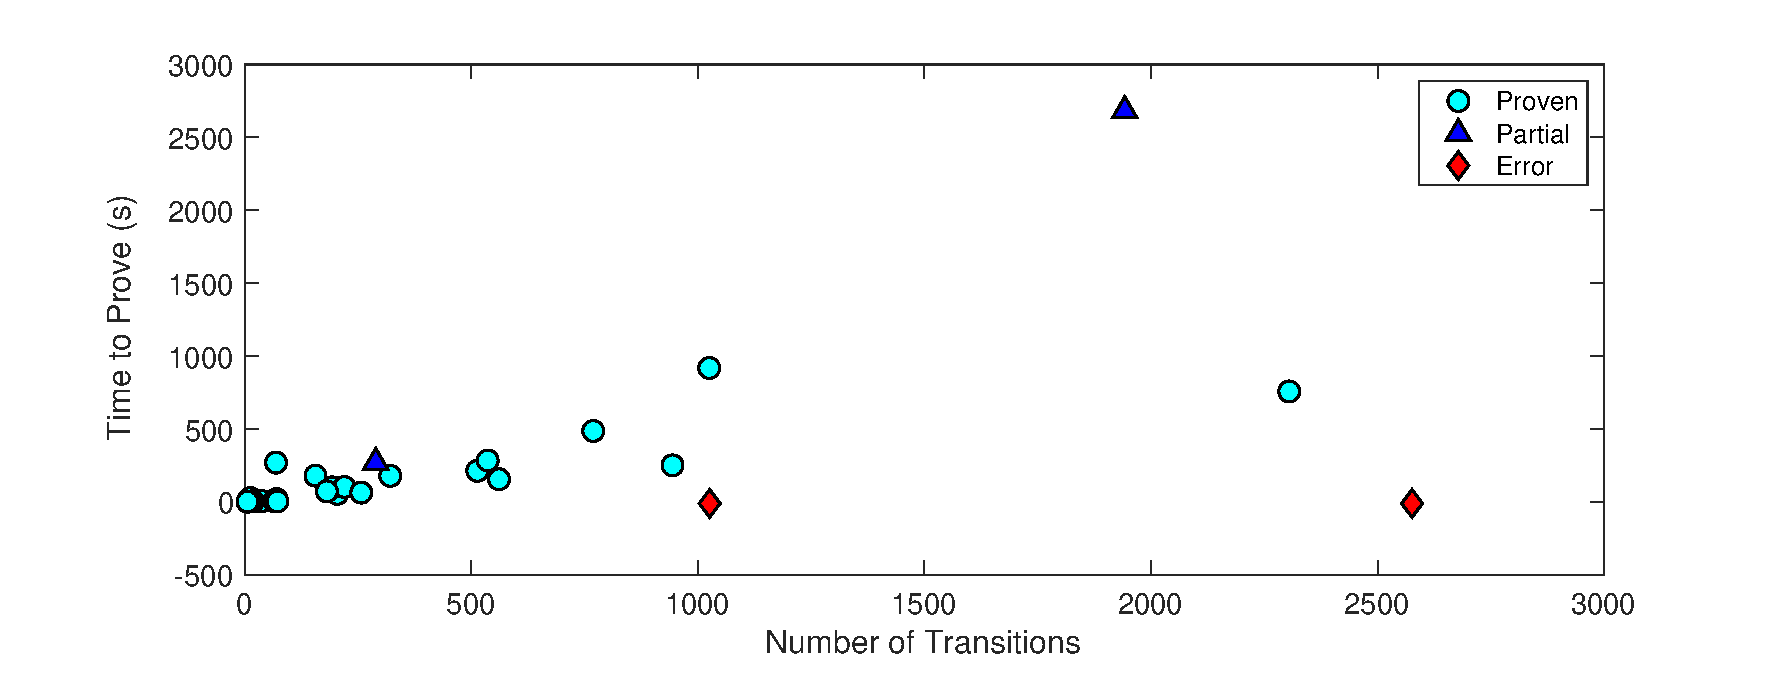
\includegraphics[width=\textwidth]{salty.eps}
\caption{Timing results for example controllers in SPARK as a function of number of transitions in the Moore machine representing the controller. Examples marked ``proven'' were fully verified, examples marked ``partial'' were partially verified, and examples marked ``error'' were too big to analyze.}
\label{fig:timingResults}
\end{figure}


%%%%%%%%%%%%%%%%%%%%%%%%%%%%%%%%%%%%%%%%%%%%%%%%%%%%%%%%%%%%%%%%%%%%%%%%%%%%%%%%
% Lessons Learned
%%%%%%%%%%%%%%%%%%%%%%%%%%%%%%%%%%%%%%%%%%%%%%%%%%%%%%%%%%%%%%%%%%%%%%%%%%%%%%%%
\section{Lessons Learned}
\label{sec:lessonsLearned}

Throughout the process of synthesizing and attempting to verify controllers in SPARK, we learned several lessons, 
both about SPARK and about some of the finer points of GR(1) specifications.

In terms of encoding SPARK controllers for verification, we originally tried to 
mirror the approach taken in other Salty language targets by building a static lookup table for state transitions. 
To do this, we tried to create an array of \lstinline{Formal_Hashed_Maps} indexed by \lstinline{State_Num}, where keys 
were derived from environment input values and used to look up the next \lstinline{State_Num} and corresponding system output values. 
Ghost functions consisting of nested quantified expressions were used to assert that in each state, initial and transition properties held 
according to values stored in the current state's hashed map and the outputs of next states. 
These functions comprised the post-condition of a function that initialized the controller's lookup table. 
The body of the \lstinline{Move} procedure simply retrieved the outputs and next state from the lookup table 
using its stored \lstinline{State_Num} and \lstinline{Environment} input.
The public portion of the SPARK specification was largely unchanged.
This approach was only able to prove the smallest of examples in a reasonable amount of time. 

While the use of formal containers was intuitive, they are more complex to reason about with respect to proof 
because they require reasoning about models of the containers and the effects of container operations. 
Encoding the lookup table as a case statement is more straightforward, because for instance, 
it is ``obvious'' to the underlying solvers that state transitions are static and that a transition exists for every possible input, since 
case statements must be exhaustive. 
%When building a lookup table represented as a formal container, one can imagine the provers would have to do additional reasoning 
%to ensure that all possible transitions are defined for each state, and no entries are ever deleted or added to the container at other points in the code. 
Encoding the \lstinline{Move} procedure as a case statement still has some issues, mainly that 
(1) the generated code can be quite long, leading to memory errors when trying to prove the subprogram with SPARK, and
(2) when proving the postcondition, since the solvers prove all cases at the same time and the number of cases grows 
exponentially with the number of inputs, sometimes the solvers are not able to prove the postcondition.
A solution to both problems could be to split the \lstinline{Move} procedure into several smaller procedures. %, e.g. splitting on the number of states 
% in a manner similar to a classic programmer splitting large subprograms into smaller ones. 
This would allow SPARK to apply its modular analysis on several smaller procedures, thus enabling the proof on larger files. 
We are currently investigating ways to split up the procedure that does not accidentally create more difficulties for the solvers.

Analysis with SPARK did reveal unexpected behaviors in two controllers synthesized from our corpus of examples. 
In particular, these controllers contained empty case statements in the \lstinline{Move} procedure. 
Upon inspection of the Slugs output, these corresponded to states with no successors. 
Upon inspection of the specifications, we found that these two examples\footnote{Salty's vip\_orig.salt and Anzu's arbiter.salt} had 
environment transition terms that allowed the environment to produce an input that would always cause 
the environment to violate its own specification on the next time step. 
These specifications had the form $\always \lnot p$ instead of $\always \lnext \lnot p$. 
The distinction is important. 
In the former case, the environment can choose $p$ for its next input and not violate the specification on the current time step. 
However, it violates it on the next time step when $p$ becomes the ``current'' value instead of the ``next'' value. 
The latter case does not allow $p$ on the next time step, and so it also cannot hold on future ``current'' steps. 
Generally, specifications should follow the latter form, 
and this was indeed an error in these specifications, so we fixed them.
However, we also modified Salty to put \lstinline{raise Program_Error} for such cases and checked 
that we were still able to prove $\varphi_e \limplies \varphi_s$ for these examples  
(since reaching these cases would require violating the precondition $\varphi_e$ on the environment). 
We found that in other Salty language targets, procedures equivalent to \lstinline{Move} would have raised random runtime exceptions 
in such cases due to empty entries in their lookup tables.

Based on our first round of SPARK analysis, we also found some examples in our database that did not have any inputs, 
i.e. they essentially amounted to synthesizing a system independent of an environment. 
In those cases, we had specifications for a non-existent environment that were vacuous, 
and this was causing SPARK to take an abnormally long amount of time to verify these controllers, given their relatively small size. 
These controllers were did not have errors per se, 
but they were inefficiently encoded. 
We modified Salty to handle such cases by removing the environment, functions over the environment, and
all references to the environment in all pre- and postconditions.
This greatly decreased verification time and also reduced the size and increased the efficiency of the code.

%%%%%%%%%%%%%%%%%%%%%%%%%%%%%%%%%%%%%%%%%%%%%%%%%%%%%%%%%%%%%%%%%%%%%%%%%%%%%%%%
% CONCLUSIONS
%%%%%%%%%%%%%%%%%%%%%%%%%%%%%%%%%%%%%%%%%%%%%%%%%%%%%%%%%%%%%%%%%%%%%%%%%%%%%%%%
\section{Conclusions}
\label{sec:conclusions}

We were able to successfully use SPARK to verify safety and transition properties of moderately sized controllers 
synthesized from GR(1) specifications by the tool Salty. 
Encoding the controllers and all of the annotations necessary for these controllers to prove automatically was relatively straighforward. 
The act of performing ``end-to-end'' verification with SPARK on such controllers was valuable because (1) it revealed implementation errors for certain 
types of specifications that result in random runtime errors in other Salty target languages, and (2) it revealed cases in which controllers were inefficiently encoded, i.e. when there is no environment.

In terms of future work, we can potentially improve the scalability of our approach by decomposing the \lstinline{Move} procedure 
into several subprocedures, as discussed in the previous section. 
We are also interested in expressing and proving liveness properties. 
Liveness properties will be more challenging to verify because they necessarily require reasoning about future states. 
Verifying system liveness in SPARK will require something like encoding a lookahead and showing that certain states will inevitably be reached 
when the environment satisfies its specification, which can also include liveness terms. 
This is likely to result in complex first-order formulas with alternating quantification over time, which are 
notoriously hard to handle for automated solvers, so discharging the resulting proof obligations may prove to be a challenge.
To tackle this issue, collaboration with a model checker performing verification at the level of the input language might be appropriate.

%
% ---- Bibliography ----
%
% BibTeX users should specify bibliography style 'splncs04'.
% References will then be sorted and formatted in the correct style.
%
\newpage
\bibliographystyle{splncs04}
\bibliography{bibfile}

\end{document}
